\documentclass{beamer}

% Solarized Theme
\usecolortheme[light, accent=orange]{solarized}
\beamertemplatenavigationsymbolsempty

% Packages
\usepackage[T1]{fontenc}
\usepackage[utf8]{inputenc}
\usepackage[english]{babel}


\usepackage{amsmath,amssymb,lmodern}
\usepackage{caption}
\usepackage{graphicx}
\usepackage{rotating}
\usepackage{tikz}
\usepackage{tikzsymbols}
\usetikzlibrary{positioning, math, automata}

\begin{document}

 
\begin{frame}
    \frametitle{Ambulance Decision Game}
    \centering
    % Ambulances Image
    \begin{minipage}{.45\textwidth}
        \centering
        \begin{figure}
            
\includegraphics[width=\textwidth]{picture/main.jpg}
        \end{figure}
    \end{minipage}
    \begin{minipage}{.45\textwidth}
        \centering
        \begin{figure}
            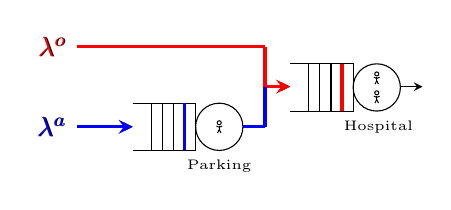
\begin{tikzpicture}[>=stealth, scale=0.4],
                % the rectangle with vertical rules (Queue 1)
                \draw (0,0) -- ++(2cm,0) -- ++(0,-1.5cm) -- ++(-2cm,0);
                \foreach \i in {1,...,4}
                \draw (2cm-\i*10pt,0) -- +(0,-1.5cm);
                
                % the circle (Queue 1)
                \draw (2.75,-0.75cm) circle [radius=0.75cm];
        
                % the rectangle with vertical rules (Queue 2)
                \draw (5,1.25) -- ++(2cm,0) -- ++(0,-1.5cm) -- ++(-2cm,0);
                \foreach \i in {1,...,4}
                \draw (7cm-\i*10pt,1.25) -- +(0,-1.5cm);
        
                % the circle (Queue 2)
                \draw (7.75,0.5) circle [radius=0.75cm];
        
                % the arrows and labels (Queue 1+2)
                \draw[->] (8.5,0.525) -- +(20pt,0);
                \node[align=center] at (1cm,-2cm) {};
                \node[align=center] at (2.75cm,-2cm) {\tiny{Parking}};
                \node[align=center] at (6cm,-0.75cm) {};
                \node[align=center] at (7.8cm,-0.75cm) {\tiny{Hospital}};
                
                % Ambulance lines
                \draw[<-] (0,-0.75) -- +(-50pt,0) node[left] {\( \lambda^a \)};
                \draw[-] (3.5,-0.75) -- +(20pt,0);
                \draw (4.2, 0.525) -- (4.2, -0.75);
    
                % Others lines
                \draw (4.2, 1.8) -- +(-169.5pt,0) node[left] {\( \lambda^o \)};
                \draw (4.2, 1.8) -- (4.2, 0.525);
                \draw[->] (4.2, 0.525) -- (5, 0.525);  
    
                % Animations
                \node[draw=none] at (7.75,0.8) {\scriptsize{\Strichmaxerl[1]}};
                \node[draw=none] at (7.75,0.2) {\scriptsize{\Strichmaxerl[1]}};
                \draw[red, very thick] (4.2, 1.8) -- +(-169.5pt,0) node[left] {\( \lambda^o \)};
                \draw[red, very thick] (4.2, 1.8) -- (4.2, 0.525);
                \draw[->, red, very thick] (4.2, 0.525) -- (5, 0.525);
                \draw[-, blue, very thick] (3.5,-0.75) -- +(20pt,0);
                \draw[blue, very thick] (4.2, 0.525) -- (4.2, -0.75);
                \draw[<-, blue, very thick] (0,-0.75) -- +(-50pt,0) node[left] {\( \lambda^a \)};
                \node[draw=none] at (2.75,-0.75) {\scriptsize{\Strichmaxerl[1]}};
                \draw[blue, very thick] (2cm-10pt,0) -- +(0,-1.5cm);
                \draw[red, very thick] (7cm-10pt,1.25) -- +(0,-1.5cm);
            \end{tikzpicture}
            \caption*{\scriptsize{Queueing Model}}
        \end{figure}
    \end{minipage}


    % Markov Chain
    \begin{minipage}{.45\textwidth}
        \centering
        \vspace{1cm}
        \begin{figure}
            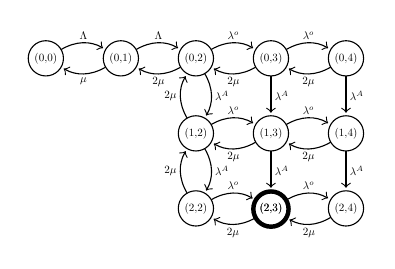
\begin{tikzpicture}[-, node distance = 0.5cm, auto, every node/.style={scale=0.4}]
                \node[state] (one) {(0,0)};    
                \node[state, right=of one] (two) {(0,1)};    
                \node[state, right=of two] (three) {(0,2)};    
                \node[state, right=of three] (four) {(0,3)};

                \node[state, right=of four] (five) {(0,4)};
                \node[state, below=of three] (three_one) {(1,2)};
                \node[state, below=of three_one] (three_two) {(2,2)};
    
                \node[state, below=of four] (four_one) {(1,3)};    
                \node[state, below=of four_one] (four_two) {(2,3)};
                \node[state, ultra thick, below=of four_one] (four_two) {(2,3)};
    
                \node[state, below=of five] (five_one) {(1,4)};
                \node[state, below=of five_one] (five_two) {(2,4)};
    
                \draw[every loop]
                    (one) edge[bend left] node {\( \Lambda \)} (two)
                    (two) edge[bend left] node {\( \mu \)} (one)
                    (two) edge[bend left] node {\( \Lambda \)} (three)
                    (three) edge[bend left] node {\( 2\mu \)} (two)
                    (three) edge[bend left] node {\( \lambda^o \)} (four)
                    (four) edge[bend left] node {\( 2\mu \)} (three)
                    (four) edge[bend left] node {\( \lambda^o \)} (five)
                    (five) edge[bend left] node {\( 2\mu \)} (four)
                    (three) edge[bend left] node {\( \lambda^A \)} (three_one)
                    (three_one) edge[bend left] node {\( 2\mu \)} (three)
                    (three_one) edge[bend left] node {\( \lambda^o \)} (four_one)
                    (four_one) edge[bend left] node {\( 2\mu \)} (three_one)
                    (four_one) edge[bend left] node {\( \lambda^o \)} (five_one)
                    (five_one) edge[bend left] node {\( 2\mu \)} (four_one)
                    (four) edge node {\( \lambda^A \)} (four_one)
                    (five) edge node {\( \lambda^A \)} (five_one)
                    (three_one) edge[bend left] node {\( \lambda^A \)} (three_two)
                    (three_two) edge[bend left] node {\( 2\mu \)} (three_one)
                    (four_one) edge node {\( \lambda^A \)} (four_two)
                    (five_one) edge node {\( \lambda^A \)} (five_two)
                    (three_two) edge[bend left] node {\( \lambda^o \)} (four_two)
                    (four_two) edge[bend left] node {\( 2\mu \)} (three_two)
                    (four_two) edge[bend left] node {\( \lambda^o \)} (five_two)
                    (five_two) edge[bend left] node {\( 2\mu \)} (four_two)
                    ;       
            \end{tikzpicture}
            \caption*{\scriptsize{Markov chain}}
        \end{figure}
    \end{minipage}
    \begin{minipage}{.51\textwidth}
        \centering
        
\includegraphics[width=1.2\textwidth, height=.43\textheight]{game_plot/main.pdf}
    \end{minipage}
\end{frame}
\end{document}